%-----------------------------------------
% Note: Use pdflatex to process this file.
%-----------------------------------------

%\documentclass{article}
\documentclass{hitec}

\usepackage{setspace}
\usepackage{graphicx}
\usepackage{moreverb}    % Defines {listing} environment.
\usepackage{amsmath, amsthm, amssymb, amsbsy, mathtools}
\usepackage{alltt}
\usepackage{rotating}
\usepackage{subcaption}
\usepackage{toc-bmad}
\usepackage{xspace}
%%\usepackage{makeidx}
\usepackage[section]{placeins}   % For preventing floats from floating to end of chapter.
\usepackage{longtable}  % For splitting long vertical tables into pieces
\usepackage{index}
\usepackage{multirow}
\usepackage{booktabs}   % For table layouts
\usepackage{yhmath}     % For widehat
\usepackage{xcolor}      % Needed for listings package.
\usepackage{listings}
\usepackage[T1]{fontenc}   % so _, <, and > print correctly in text.
\usepackage[strings]{underscore}    % to use "_" in text
\usepackage[pdftex,colorlinks=true]{hyperref}   % Must be last package!

%----------------------------------------------------------------

\newcommand{\extref}[1]{$\S$\ref*{#1}}   % No hyperlink. For external refs. \extref
\newcommand{\comma}{\> ,}
\newcommand{\period}{\> .}
\newcommand{\wt}{\widetilde}
\newcommand{\grv}{\textasciigrave}
\newcommand{\hyperbf}[1]{\textbf{\hyperpage{#1}}}
\newcommand{\Ss}{\(^*\)}
\newcommand{\Dd}{\(^\dagger\)}

\newcommand{\AND}{&& \hskip -17pt\relax}
\newcommand{\CR}{\\}
\newcommand{\CRNO}{\nonumber \\}
\newcommand{\dstyle}{\displaystyle}

\newcommand{\Begineq}{\begin{equation}}
\newcommand{\Endeq}{\end{equation}}
\newcommand{\NoPrint}[1]{}

\newcommand{\pow}[1]{\cdot 10^{#1}}
\newcommand{\Bf}[1]{{\bf #1}}
\newcommand{\bfr}{\Bf r}

\newcommand{\bmad}{{\sl Bmad}\xspace}
\newcommand{\tao}{{\sl Tao}\xspace}
\newcommand{\mad}{{\sl MAD}\xspace}
\newcommand{\cesr}{{\sl CESR}\xspace}

\newcommand{\sref}[1]{\S\ref{#1}}
\newcommand{\Sref}[1]{Sec.~\sref{#1}}
\newcommand{\cref}[1]{Chapter~\ref{#1}}

\newcommand{\Newline}{\hfil \\ \relax}

\newcommand{\eq}[1]{{(\protect\ref{#1})}}
\newcommand{\Eq}[1]{{Eq.~(\protect\ref{#1})}}
\newcommand{\Eqs}[1]{{Eqs.~(\protect\ref{#1})}}

\newcommand{\vn}{\ttcmd}           % For variable names
\newcommand{\vni}{\ttcmdindx}
\newcommand{\cs}{\ttcmd}           % For code source
\newcommand{\cmd}{\ttcmd}          % For Unix commands
\newcommand{\rn}{\ttcmd}           % For Routine names
\newcommand{\tn}{\ttcmd}           % For Type (structure) names
\newcommand{\bn}[1]{{\bf #1}}       
\newcommand{\toffset}{\vskip 0.01in}
\newcommand{\rot}[1]{\begin{rotate}{-45}#1\end{rotate}}

\newcommand{\data}{{\mbox{data}}}
\newcommand{\reference}{{\mbox{ref}}}
\newcommand{\model}{{\mbox{model}}}
\newcommand{\base}{{\mbox{base}}}
\newcommand{\design}{{\mbox{design}}}
\newcommand{\meas}{{\mbox{meas}}}
\newcommand{\var}{{\mbox{var}}}

\newcommand\ttcmd{\begingroup\catcode`\_=11 \catcode`\%=11 \dottcmd}
\newcommand\dottcmd[1]{\texttt{#1}\endgroup}

\newcommand\ttcmdindx{\begingroup\catcode`\_=11 \catcode`\%=11 \dottcmdindx}
\newcommand\dottcmdindx[1]{\texttt{#1}\endgroup\index{#1}}

\newcommand{\St}{$^{st}$\xspace}
\newcommand{\Nd}{$^{nd}$\xspace}
\newcommand{\Th}{$^{th}$\xspace}
\newcommand{\B}{$\backslash$}
\newcommand{\W}{$^\wedge$}

\newcommand{\cbar}[1]{\overline C_{#1}}

\newlength{\dPar}
\setlength{\dPar}{1.5ex}

\newenvironment{example}
  {\vspace{-3.0ex} \begin{alltt}}
  {\end{alltt} \vspace{-2.5ex}}

\newcommand\Strut{\rule[-2ex]{0mm}{6ex}}

\newenvironment{Itemize}
  {\begin{list}{$\bullet$}
    {\addtolength{\topsep}{-1.5ex} 
     \addtolength{\itemsep}{-1ex}
    }
  }
  {\end{list} \vspace*{1ex}}

\newcommand{\Section}[1]{\section{#1}\indent\vspace{-3ex}}

\newcommand{\SECTION}[1]{\section*{#1}\indent\vspace{-3ex}}

% From pg 64 of The LaTex Companion.

\newenvironment{ventry}[1]
  {\begin{list}{}
    {\renewcommand{\makelabel}[1]{\textsf{##1}\hfil}
     \settowidth{\labelwidth}{\textsf{#1}}
     \addtolength{\itemsep}{-1.5ex}
     \addtolength{\topsep}{-1.0ex} 
     \setlength{\leftmargin}{5em}
    }
  }
  {\end{list}}


\newcommand{\BF}[1]{{\normalfont\textbf{#1}}}

\renewcommand{\ttdefault}{txtt}

\renewcommand{\textfraction}{0.1}
\renewcommand{\topfraction}{1.0}
\renewcommand{\bottomfraction}{1.0}

\settextfraction{0.9}  % Width of text
\setlength{\parindent}{0pt}
\setlength{\parskip}{1ex}
%\setlength{\textwidth}{6in}
\newcommand{\Section}[1]{\section{#1}\vspace*{-1ex}}

\newenvironment{display}
  {\vspace*{-1.5ex} \begin{alltt}}
  {\end{alltt} \vspace*{-1.0ex}}

\title{Bmad and Tao Concepts Tutorial}
\author{}
\date{David Sagan \\ June 24, 2016}
\begin{document}
\maketitle

\tableofcontents

%------------------------------------------------------------------------------
\Section{A Guide for the Perplexed}
\label{s:guide}

This is a tutorial to introduce the reader to some of the concepts that are used by the \bmad toolkit
for relativistic charged--particle and X-Ray simulations and as an initial training tutorial
for using the \tao simulation program.

It is assumed that you know something about accelerator physics. In particular it is assumed that
you know about beta functions, dispersion and closed orbits.

%------------------------------------------------------------------------------
\Section{Overview: What is Bmad? What is Tao?}
\label{s:overview}

\bmad is an open-source subroutine library for relativistic charged--particle and X-Ray simulations
in accelerators and storage rings. \bmad has been developed at Cornell University's Laboratory for
Elementary Particle Physics.  Over the years, \bmad has been used for a wide range of
charged-particle and X-ray simulations. The following list gives some idea as to the range that
\bmad has been put to use for:
\begin{display}
  Lattice design                              X-ray simulations
  Spin tracking                               Wakefields and HOMs
  Beam breakup simulations in ERLs            Touschek Simulations
  Intra-beam scattering (IBS) simulations     Dark current tracking
  Coherent Synchrotron Radiation (CSR)        Frequency map analysis
\end{display}

The advantage of \bmad over a stand-alone simulation program is that when new types of simulations
need to be developed, \bmad can be used to cut down on the time needed to develop such programs
with the added benefit that the number of programming errors will be reduced
as well. The disadvantage of \bmad is that, as a toolkit, one cannot perform any calculations
without first developing a program. To get around this, a program called \tao was developed.
\tao is a general purpose simulation program, based upon \bmad. \tao can be used to view
lattices, do Twiss and orbit calculations, nonlinear optimization on lattices, etc., etc.
Additionally, \tao's object oriented design makes it relatively easy to extend it. For
example, it can be used for orbit flattening in a machine control system.

%------------------------------------------------------------------------------
\Section{Resources}
\label{s:resources}

More information is readily available at the \bmad and \tao web site:
\begin{display}
  \url{http://www.lepp.cornell.edu/~dcs/bmad}
\end{display}
Links to the \bmad and \tao manuals can be found there as well as instructions for
downloading and setup if needed, etc.

%------------------------------------------------------------------------------
\Section{How to Use this Tutorial}

This tutorial contains a set of examples which involve running the \tao program. 
While it is not 100\% necessary that you actually run \tao with the examples, it is
definitely easier to absorb the material if you do. For instructions on installing \bmad
and \tao, please go to the \bmad web site (\sref{s:resources}).

\tao is a command line program so you will need a terminal emulator program like \vn{terminal} on a
Mac.

To find out if everything is properly setup. Issue the command
\begin{code}
> which tao
\end{code}
The response should be the location of the \tao executable which will look something like:
\begin{code}
/Users/dcs16/bmad/bmad_dist/production/bin/tao
\end{code}
If there is no response, consult your local \bmad Guru or look at the \bmad web site.

%------------------------------------------------------------------------------
\Section{Introduction to Bmad Lattices}
\label{s:bmad.intro}

The basis of any \bmad based simulation is a lattice file. So the following is a
simple example:
\begin{code}
beginning[beta_a] = 10.   ! m  a-mode beta function
beginning[beta_b] = 10.   ! m  b-mode beta function
beginning[e_tot] = 10e6   ! eV   Or can set p0c

parameter[geometry] = open      ! or closed
parameter[particle] = electron  ! Reference particle.

d: drift, L = 0.5
b: sbend, L = 0.5, g = 1    ! g = 1 / bending_radius
q: quadrupole, L = 0.6, k1 = 0.23

lat: line = (d, b, q)   ! List of lattice elements
use, lat                ! Line used to construct the lattice
\end{code}
Part I of the \bmad manual covers lattice syntax so please refer to that for information that
is not covered here.

Some comments on the above lattice:
  \begin{description}
  \item[{beginning[...], parameter[...]}] \Newline
Global parameters (parameters of the lattice that are not associated with any one given lattice
element) can be set using \vn{beginning[...]}, \vn{parameter[...]} and \vn{beam_start[...]}
constructs. See the \vn{Lattice File Global Parameters} chapter in the \bmad manual for a
complete list of parameters that can be set.
  \item[{parameter[geometry]}] \Newline
The \vn{parameter[geometry]} parameter set whether the geometry of the lattice is considered
\vn{open} like a 1-pass accelerating linac or \vn{closed} like a storage ring. If the lattice is
closed, the closed orbit is used as the reference orbit and the computed beta functions
correspond to the periodic solution. If the lattice is \vn{open}, the orbit and beta functions
are computed using the beginning orbit and beta functions as set in the lattice. The default
geometry is \vn{open} if the lattice contains an \vn{lcavity} (linac accelerating RF cavity) 
element and is \vn{closed} if no \vn{lcavity} is present.
  \item[{beginning[beta_a], beginning[beta_b]}] \Newline
The \vn{beginning[beta_a]} and \vn{beginning[beta_b]} parameters are the beta functions at beginning
of the lattice. The beginning beta functions will be only used by \bmad if the lattice geometry is
set to \vn{open}. Note: Some programs will use the labels \vn{beta_x} and \vn{beta_y} for the beta
functions. This is inaccurate since the beta functions are associated with the normal modes of
oscillation of the beam and, if there is horizontal/vertical coupling, the normal modes will not
correspond to purely horizontal and purely vertical motion. In the limit of no coupling, the
\vn{a}-mode will correspond to horizontal oscillations and the \vn{b}-mode will correspond to
vertical oscillations.
  \item[{beginning[e_tot]}] \Newline
The \vn{beginning[e_tot]} parameter sets the reference total energy at the beginning of the lattice.
Alternatively, \vn{beginning[p0c]} can be used to set the reference momentum at the beginning of the
lattice.
  \item[{parameter[particle]}] \Newline
The \vn{parameter[particle]} parameter sets the reference particle. Besides fundamental particles,
ions can be used. For example, the reference particle could be set to \vn{\#12C+3} which is triply
charged carbon-12. The default reference particles are positrons.
  \item[d, b, q] \Newline
The lattice element named \vn{d} is a drift element. That is, a field free region. The \vn{b} is a
dipole bend and \vn{q} has a quadrupole element. See the \vn{Elements} chapter in the \bmad manual
for more details.
  \item[lat: line = (...)] \Newline
A lattice consists of an ordered list of elements that the beam goes through. \vn{lines} are used
to define this ordered list. In this instance a line called \vn{lat} contains the elements
\vn{d}, \vn{b}, and \vn{q} in that order. 
See the \vn{Beam lines and Replacement Lists} chapter of the \bmad manual for more details.
  \item[use, lat] \Newline
The \vn{use} statement in a lattice file identifies the particular line used to construct the
lattice. This is needed since a lattice file may define multiple lines and lines can contain
sub-lines, etc.
  \end{description}

[Note: the above discussion assumes that the lattice has only one \vn{branch}. Branches will be
discussed in more detail later.]

%------------------------------------------------------------------------------
\Section{Starting Tao}
\label{s:tao.start}

\begin{figure}[tb]
  \centering
  \begin{subfigure}[b]{0.47\textwidth}
    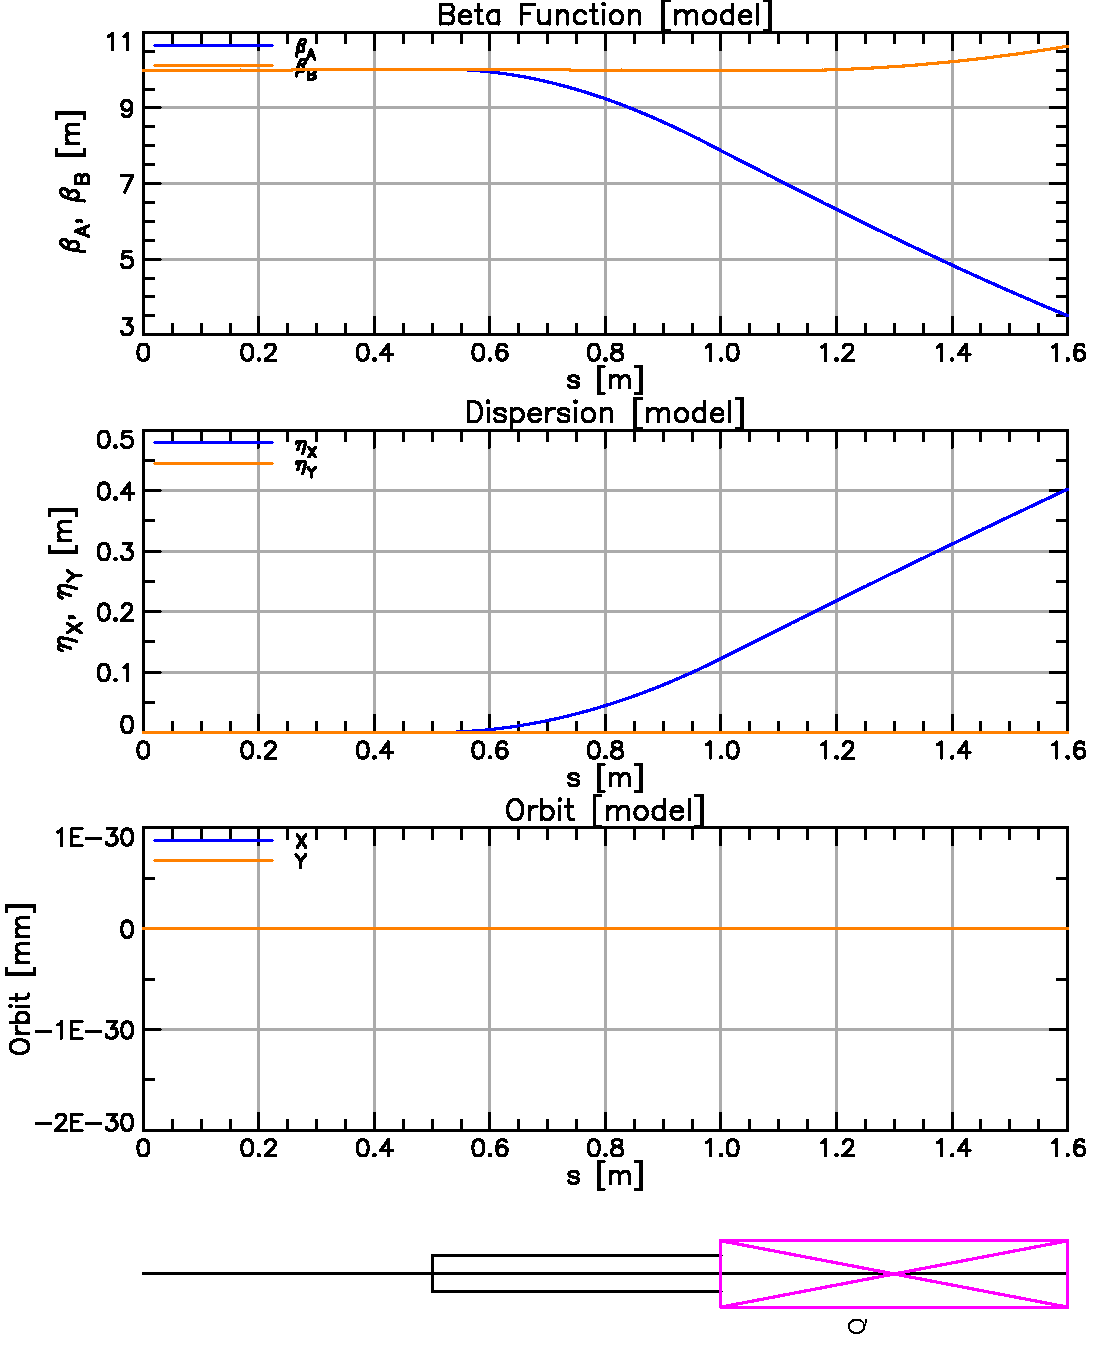
\includegraphics[width=\textwidth]{lat-init.pdf}
    \caption{Initial graphics when \tao is run with the \vn{lat.bmad} lattice file.}
    \label{f:lat.init}
  \end{subfigure}
  \hfil
  \begin{subfigure}[b]{0.47\textwidth}
    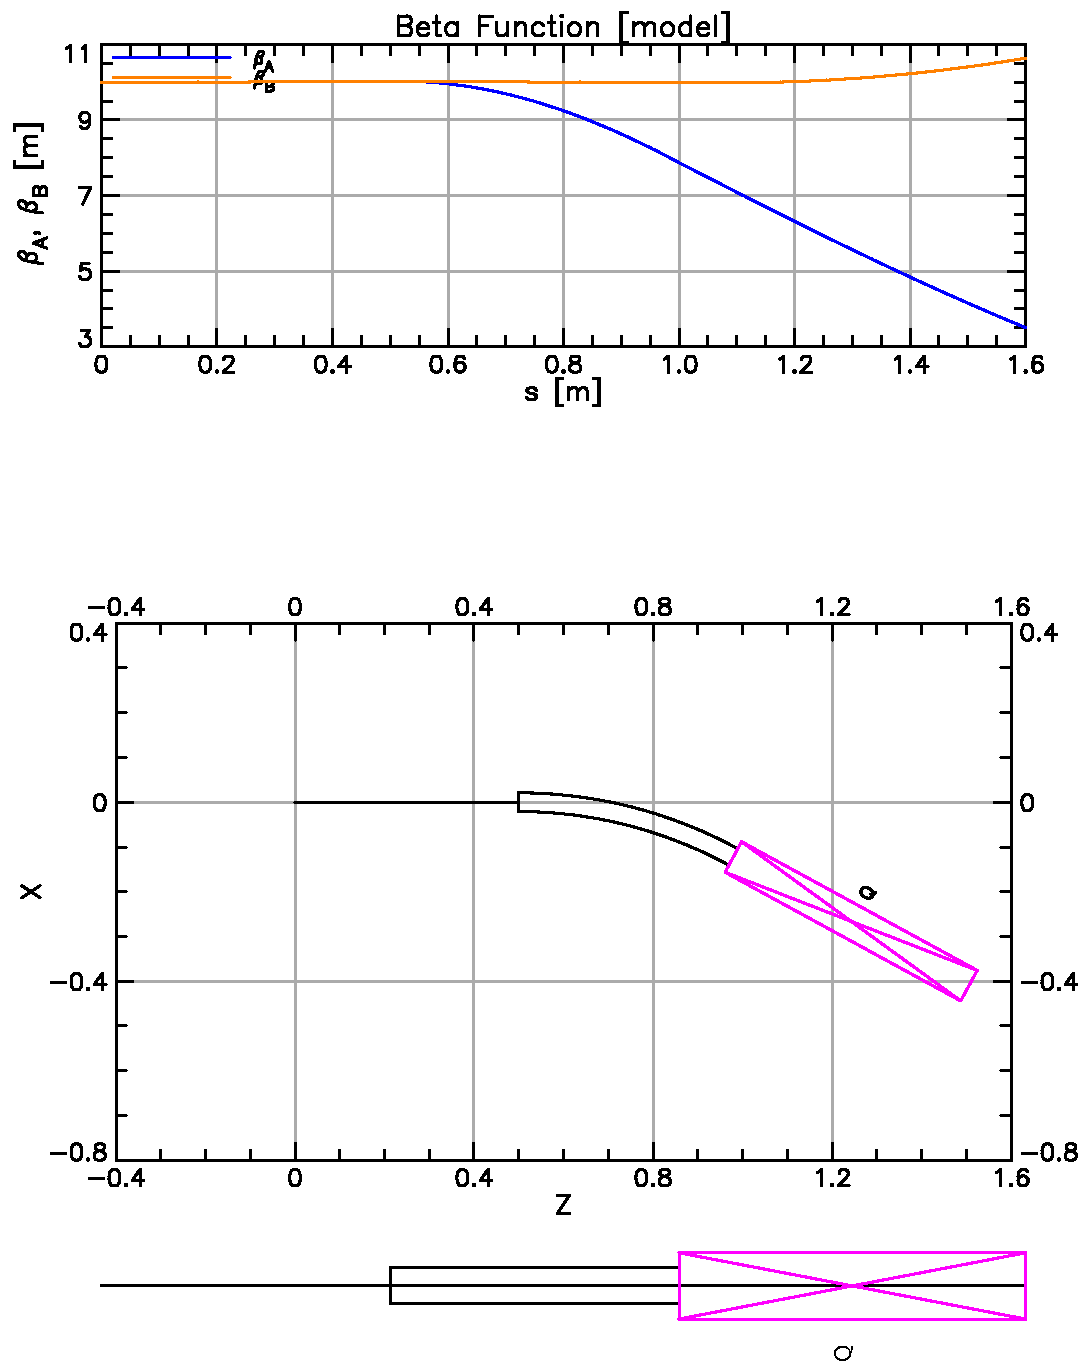
\includegraphics[width=\textwidth]{lat-floor.pdf}
    \caption{Graphics after a \vn{place r22 floor_plan} command.}
    \label{f:lat.floor}
  \end{subfigure}
  \caption{Example \tao graphics.}
\end{figure}

To run, \tao needs a lattice file as input. For this example, the lattice file shown in
section~\sref{s:bmad.intro} will be used. Copy the lattice into a file and called \vn{lat.bmad}.
Make sure that the directory from which you are running \tao does not have a file called
\vn{tao.init} since this file can affect things (more on that later). Run \tao with the command:
\begin{code}
> tao -lat lat.bmad
\end{code}
\tao should open a window for plotting. If this window is too large for your screen, you can adjust
the size of the plotting window by using the \vn{-geometry} option. Example:
\begin{code}
> tao -lat lat.bmad -geom 400x400
\end{code}
Consult the \tao manual for a list of command line arguments or use the command:
\begin{code}
> tao -help
\end{code}

In your terminal window there should be a \vn{Tao>} prompt where you can type \tao commands.
Additionally, a plot window is created. When you run tao with the above lattice, the plot window
should look like figure~\ref{f:lat.init}. The default is to have three plots: beta, dispersion, and
orbit, along with what is called a \vn{lat_layout} plot (at the bottom of the window) that
graphically shows the lattice elements. Note: If you do not want \tao to display the plot window,
use the \vn{-noplot} option on the command line.

%----------------------------------------------------------
\Section{Tao: Getting Help}

\vn{To Do}: Start \tao as explained in section~\sref{s:tao.start} with the lattice file
\vn{lat.bmad} of section~\sref{s:bmad.intro} and experiment with the \vn{help} command
as you read this section.

To get a list of Tao commands use the \vn{help} command
\begin{code}
Tao> help

Type 'help <command>' for help on an individual command
Available commands:
  alias                             read
  call                              restore
  change                            reinitialize
  clip                              run_optimizer
  continue                          scale
  derivative                        set
  end_file                          show
  exit                              single_mode
  flatten                           spawn
... etc...
\end{code}
[For brevity's sake, \vn{... etc...} is used when the output has been truncated.]

\tao commands are documented in the \vn{Tao Line Mode Commands} chapter of the \tao manual.
This same documentation can be displayed using the \vn{help <command>} command where
\vn{<command>} is the name of a command. Example:
\begin{code}
Tao> help set

The "set" command is used to set values for data,
variables, etc. Format:
  set beam_init {n@}<component> = <value>
  set beam_start {n@}<coordinate> = <value>
  set bmad_com <component> = <value>
  set csr_param <component> = <value>
  set curve <curve> <component> = <value>
  set data <data_name>|<component> = <value>
  set default <parameter> = <value>
  set element <element_list> <attribute> = <value>
  set floor_plan <component> = <value>
  set geodesic_lm <component> = <value>
... etc...

Also see the "change" command . The "change" command is specialized
for varying real parameters while the "set" command is more general.

... etc...

Use the command:
  help set <what>
to obtain more information on a particular set subtopic. Example:
  help set plot
\end{code}

Some commands are complicated enough so that there is a second level to the help on these commands.
The \vn{set} command is an example of such a command. Thus you can type \vn{help set curve} for
help on setting plotting curve parameters.

%----------------------------------------------------------
\Section{Tao: Show This and Show That}

\vn{To Do}: Start \tao as explained in section~\sref{s:tao.start} with the lattice file
\vn{lat.bmad} of section~\sref{s:bmad.intro} and experiment with the \vn{show} command as you read
this section. [Alternatively, use one of the more complicated lattices in the
\vn{examples/lattice_file_examples} directory (if you do not know where this directory is, consult
your local \bmad Guru).]

\subsection{To Show a List of Elements in the Lattice}

To show the elements in the lattice use the command \vn{show lattice}:
{\small
\begin{code}
 Tao> show lat
      Values at End of Element:
 Index  name      key                       s       l    beta     phi ...
                                                            a       a ...
     0  BEGINNING Beginning_Ele         0.000     ---   10.00   0.000 ...
     1  D         Drift                 0.500   0.500   10.03   0.050 ...
     2  B         Sbend                 1.000   0.500    7.87   0.104 ...
     3  Q         Quadrupole            1.600   0.600    3.50   0.217 ...
     4  END       Marker                1.600   0.000    3.50   0.217 ...
 Index  name      key                       s       l    beta     phi ...
                                                            a       a ...
      Values at End of Element:
\end{code}}

Notice that \bmad adds two extra elements to the lattice. A zero length beginning element called \vn{BEGINNING}
and a zero length marker element at the end called \vn{END}.

The "show lat" command, like many other commands, has lots of optional parameters to customize the
table of information printed:

{\small
\begin{code}
Tao> help show lat

Syntax:
  show lattice {-0undef} {-all} {-attribute <attrib>} {-base}
      {-blank_replacement <string>}  {-branch <name_or_index>}
      {-custom <file_name>} {-design} {-floor_coords} {-lords} {-middle}
      {-no_label_lines} {-no_tail_lines} {-no_slaves} {-orbit} 
      {-remove_line_if_zero <column #>} {-s <s1>:<s2>} {-tracking_elements}
      {<element_list>}

Show a table of Twiss and orbit data, etc. at the specified element locations. 
The default is to show the parameters at the exit end of the elements. 
... etc...
\end{code}}

%----------------------------------------------------------
\subsection{To Show the Attributes of a Lattice Element}

Use the \vn{show element} command to show the attributes of a particular lattice elements. Example:
{\small
\begin{code} 
Tao> show ele b   ! or: show ele 2

 Element #                2
 Element Name: B
 Key: Sbend
 Sub Key: SBend
 S_start, S:    0.500000,    1.000000
 Ref_time:  3.340005E-09

 Attribute values [Only non-zero/non-default values shown]:
    1   L                            =  5.0000000E-01 m
    6   G                            =  1.0000000E+00 1/m
    8   RHO                          =  1.0000000E+00 m
   13   SPIN_FRINGE_ON               =  T (1)
   19   E1                           =  0.0000000E+00 rad
   20   E2                           =  0.0000000E+00 rad
   29   L_SAGITTA                    =  3.1087578E-02 m
		 ... etc...

Twiss at end of element:
                          A              B            Cbar    ...
  Beta (m)         7.87064432     9.99974729  |   0.00000000  ...
  Alpha            3.93634109     0.20027369  |   0.00000000  ...
  Gamma (1/m)      2.09573455     0.10401358  |   Gamma_c =   ...
  Phi (rad)        0.10395730     0.09991742            X     ...
  Eta (m)          0.12241744     0.00000000     0.12241744   ...
  Etap             0.48187421     0.00000000     0.48187421   ...

Orbit:  Positron   State: Alive
         Position[mm] Momentum[mrad]        Spin   |
  X:       0.00000000     0.00000000               | Particle [sec]: ...
  Y:       0.00000000     0.00000000               | Part-Ref [sec]: ...
  Z:       0.00000000     0.00000000               | (Ref-Part)*Vel  ...
\end{code}}
Note: By default, only non-zero attributes are shown. Use the -all option to see all the attributes.

%----------------------------------------------------------
\subsection{To Show a List of Elements Using Wild Cards}

Use the \vn{show element} with a wild card character to show all elements matching a particular
pattern. Wild card character are:
{\small
\begin{code}
"*" -- Matches to any number of characters.
"%" -- Matches to any single character.
\end{code}}
The general syntax is:
{\small
\begin{code}
show element <element_type>::<name_with_wild_card_characters>
\end{code}}

For example, to show all elements whose name begins with "Q" the command is:
{\small
\begin{code}
Tao> show ele q*

         1  Q                                                1.000
Number of Matches: 1
\end{code}}

Or to show all sbend elements the command is:
{\small
\begin{code}  
Tao> show ele sbend::*

         2  B                                                2.000
Number of Matches: 1
\end{code}}

%----------------------------------------------------------
\Section{Introduction to Plotting in Tao}

\vn{To Do}: Start \tao as explained in section~\sref{s:tao.start} with the lattice file
\vn{lat.bmad} of section~\sref{s:bmad.intro} and experiment with the plotting as shown 
in this section.

%----------------------------------------------------------
\subsection{Plot Page Parameters}

\begin{figure}[tb]
  \centering
  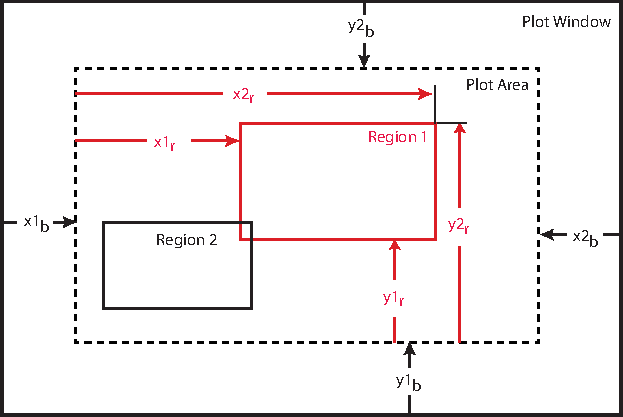
\includegraphics[width=0.7\textwidth]{plot-page.pdf}
  \caption{The plot window is divided up into a number of rectangular \vn{regions} into
which a plot \vn{template} can be placed. Regions can overlap.}
  \label{f:plot.regions}
\end{figure}


The plot window has a number of parameters that can be displayed using the \vn{show plot}
command:

{\small
\begin{code}
Tao> show plot
plot_page parameters:
  %size                         = 500     600
  %n_curve_pts                  = 401
  %text_height                  = 12.000
... etc...

Templates:
   Plot                                    Description
   ----------------------------            -------------------
   alpha                                   Twiss alpha function
   b_div_curl                              Magnetic Field Divergence and Curl.
   b_field                                 Magnetic Field Along Orbit
   beta                                    Twiss beta function
   bunch_sigma_xy                          Bunch transverse sigmas
   bunch_R1_R2                             Bunch phase space plot.
   cbar                                    Cbar coupling matrix
   dbeta                                   Chromatic normalized beta beat
... etc...

                                               Location on Page
Plot Region         <-->  Plot                 x1    x2    y1    y2
-----------               -----------------------------------------
layout              <-->  lat_layout          0.00  1.00  0.00  0.15
r11                 <-->                      0.00  1.00  0.15  1.00
r12                 <-->                      0.00  1.00  0.58  1.00
r22                 <-->                      0.00  1.00  0.15  0.58
r13                 <-->  beta                0.00  1.00  0.72  1.00
r23                 <-->  dispersion          0.00  1.00  0.43  0.72
r33                 <-->  orbit               0.00  1.00  0.15  0.43
r14                 <-->                      0.00  1.00  0.79  1.00
... etc...
\end{code}}
The output of the \vn{show plot} is divided into three sections. The top section
shows some parameters like the size of the plot window. Use the \vn{set plot_page}
command to change these parameters. 

The middle section of the output of the \vn{show plot} command shows plot \vn{templates}.
Plot templates specify parameters for drawing plot. For example, how many graphs are
associated with a plot (in the plots of Figure.~\ref{f:init.lat} there are one graph per plot)
and how many curves per graph there are. \tao defines a set of default templates and custom
ones can be defined by constructing the appropriate initialization file. Directions for
constructing templates are given in the \vn{Initializing Plotting} section of the \vn{Tao
Initialization} chapter of the \tao manual.

The bottom section of the output of the \vn{show plot} command shows the plot \vn{regions} of the
plot window along with associated plots. The plot regions are rectangular regions of the plot window
into which a plot can be placed as illustrated in Figure~\ref{f:plot.regions}.  See the
\vn{Initializing Plotting} section of the \vn{Tao Initialization} chapter of the \tao manual. for
more details. With the present example, there are four regions that have plot. The \vn{r13} region
has a \vn{beta} plot, etc.


%----------------------------------------------------------
\subsection{Placing Plots}

The \vn{place} command is used to place a \vn{template} plot into a plot region. Example:
{\small
\begin{code}
Tao> place r22 floor_plan
\end{code}}
This places a \vn{floor_plan} plot in the \vn{r22} region.
The result is shown in Figure~\ref{f:lat.floor}. Plots associated with other regions
that overlap the region that is used in the \vn{place} command are erased. 

Example place commands:
{\small
\begin{code}
Tao> place r22 none    ! Clear a region
Tao> place * none      ! Clear all regions
\end{code}}

%----------------------------------------------------------
\subsection{Scaling Plots}

Plots can be scalled vertically using the \vn{scale} command:
{\small
\begin{code}
Tao> scale beta 0 20  ! Set y_min = 0, y_max = 20
Tao> scale r22 0 20   ! Same as above if beta plot in r22 region
Tao> scale beta       ! Tao will calculate nice bounds
Tao> scale all        ! "all" = all plots
Tao> scale            ! Same as "scale all"
\end{code}}

The \vn{x_scale} command can be used to scale the horizontal axis and
the \vn{xy_scale} command can be used to simultaneously scale the x and y axis.
{\small
\begin{code}
Tao> x_scale beta 0.8 1.0   ! Scale horizontal axis
Tao> xy_scale floor_plan    ! Combined scale and x_scale.
\end{code}}

\newpage

%----------------------------------------------------------
\Section{Model Design and Base Lattices in Tao}

When \tao runs, \tao instantiates three lattices:
\begin{description}
\item[\vn{Design Lattice}] \Newline
The \vn{design} lattice corresponds to the lattice read in from the lattice
description file(s). Parameters of this lattice are never varied.
\item[\vn{Model Lattice}] \Newline
Initially, when Tao is started, \vn{Model} = \vn{Design}. Essentially all commands to vary lattice
parameters vary parameters of this lattice.
\item[\vn{Base Lattice}] \Newline
The \vn{base} lattice is a reference lattice used so that changes in the \vn{Model} 
lattice may more easily be viewed.
\end{description}

[Technically, \tao instantiates three lattices per \vn{universe}. See below.]

%----------------------------------------------------------
\subsection{Setup}

The lattice used to illustrate things in this section is:
{\small
\begin{code}
beginning[beta_a] = 10.   ! m
beginning[beta_b] = 10.   ! m
beginning[e_tot] = 10e6   ! eV
parameter[geometry] = open  ! or closed

d: drift, L = 0.5
b: sbend, L = 0.5, g = 1, e1 = 0.01, e2 = 0.02, g_err = 0.001
q: quadrupole, L = 0.6, k1 = 0.23

lat: line = (d, b, q)
use, lat
\end{code}}

Copy this lattice to a file and run \tao with this lattice as explained in section~\sref{s:tao.start}.

%----------------------------------------------------------
\subsection{Changing Model Parameters}

To see the difference between the \vn{model} and \vn{design} lattices issue the following commands:
{\small
\begin{code}
Tao> place r23 orbit
Tao> place r13 orbit
Tao> set plot r33 component = design
Tao> set plot r13 component = model - design
Tao> scale
\end{code}}
The result is shown in 

%----------------------------------------------------------
\subsection{}

%----------------------------------------------------------
\subsection{Multiple Universes}



\end{document}